%%%%%%%%%%%%%%%%%%%%%%%%%%%%%%%%%%%%%%%%%%%%%%%%%%%%%%%%%%%%%
%% StringTemplate
%%%%%%%%%%%%%%%%%%%%%%%%%%%%%%%%%%%%%%%%%%%%%%%%%%%%%%%%%%%%%
\chapter{Aufgabe 6}
\label{sec:aufgabe6}

\subsection*{Aufgabe}
Implementieren Sie eine Java-Anwendung, die für beliebige Java-Klassen und
-Interfaces eine HTML-Seite im Format der Beispieldatei \textbf{aufgabe6.html} (siehe Moodle-Kursseite) generiert.
Leiten Sie dazu aus \textbf{aufgabe6.html} eine Stringtemplategroup-Datei \textbf{aufgabe6.stg} ab.
Die Java-Anwendung soll die gewünschten voll qualifizierten Klassen- und Interfacenamen
als Aufrufparameter bekommen und mit Hilfe der Templates die HTML-Darstellung erzeugen.

\textit{
Hinweise:
Übergeben Sie dem Wurzel-Template eine Collection oder ein Array von \textbf{Class<?>-Objekten}.
Die Objekte erzeugen Sie mit \textbf{Class.forName(String)}.
Die Stringtemplate-Bibliothek ist in der Antlr-Bibliothek enthalten,
die Sie bei vorhergehenden Aufgaben bereits verwendet haben.
}

\subsection*{Lösung}

Da aus StringTemplate heraus keine statischen Funktionen aufgerufen werden können, wie etwa \textit{c.getInterfaces()},
werden deren Werte im Voraus in einer Wrapper-Klasse als Instanzvariablen abgelegt:

\begin{code}[language=java, caption={Info Classes}, label={lst:Aufgabe6_info}]
final class ClassInfo {
    public final String name;
    public final boolean hasNoInterface;
    public final boolean hasMethods;
    public final List<String> classMethods;
    public List<InterfaceInfo> interfaces;

    public ClassInfo(Class<?> c) {
        this.name = c.getName();
        this.interfaces = Arrays.stream(c.getInterfaces()).map(InterfaceInfo::new).toList();
        this.hasNoInterface = interfaces.isEmpty();

        this.classMethods = Arrays.stream(c.getMethods())
                .map(x -> x.getReturnType() + " " + x.getName() + "(" + Arrays.toString(x.getParameterTypes()) + ")")
                .filter(o -> this.interfaces.stream().noneMatch(i -> i.methods.contains(o)))
                .toList();
        this.hasMethods = !classMethods.isEmpty();
    }
}

final class InterfaceInfo {
    public final String name;
    public final List<String> methods;

    public InterfaceInfo(Class<?> i) {
        this.name = i.getName();
        this.methods = Arrays.stream(i.getMethods()).map(
                x -> x.getReturnType() + " " + x.getName()
                        + "(" + Arrays.toString(x.getParameterTypes())
                        .replace('[', ' ').replace(']', ' ') + ")"
        ).toList();
    }
}
\end{code}
\newline

In der main Methode, werden Klassen-Objekte mit, über den \textit{args} Parameter übergebene, Klassennamen und \textit{Class.forName}
erzeugt und anschließend in unsere Wrapper-Klassen gepackt.
Eine Liste dieser Wrapper wird schließlich dem Stringtemplate übergeben und daraus die HTML-Seite generiert.

\begin{code}[language=java, caption={Main}, label={lst:Aufgabe6_main}]
public final class HtmlJavaDoc {

    public static void main(String[] args) {
        ST templ = new STGroupFile("u6/htmljavadoc.stg").getInstanceOf("docpage");

        List<? extends Class<?>> classes = Arrays.stream(args)
                .map(arg -> {
                    try {
                        return Class.forName(arg);
                    } catch (ClassNotFoundException e) {
                        throw new RuntimeException(e);
                    }
                })
                .toList();
        templ.add("p", classes.stream().map(ClassInfo::new).toList());

        String result = templ.render();
        System.out.println(result);
    }
}
\end{code}
\newline

Das Stringtemplate selbst ist in der Datei \textit{htmljavadoc.stg} abgelegt und sieht wie folgt aus:

\begin{code}[language=html, caption={String Template}, label={lst:Aufgabe6_stg}]
// htmljavadoc.stg
delimiters "$", "$"

docpage(p) ::= <<
<!DOCTYPE html>
<html lang="en">
<head>
    <meta charset="UTF-8">
    <title>Sprachkonzepte Aufgabe 6</title>

    <style>
    html { background: whitesmoke; }
    th, td { border-bottom: thin solid; padding: 4px; text-align: left; }
    td { font-family: monospace }
    </style>
</head>
<body>
<h1>Sprachkonzepte Aufgabe 6</h1>
$p:classdoc(); separator="\n"$
</body>
</html>
>>

classdoc(l) ::= <<
<h2>$l.name$</h2>
<table>
    <tbody>
        <tr>
            $if(!l.hasNoInterface)$<th>Interface</th>$endif$
            <th>Methods</th>
        </tr>
        $l.interfaces:rowdoc(); separator="\n"$
        $if(l.hasNoInterface && l.hasMethods)$<tr><td>$l.classMethods; separator="<br>"$</td></tr>$endif$
    </tbody>
</table>
>>

rowdoc(c) ::= <<
<tr>
    <td valign="top">
    $c.name$
    </td>
    <td>
        $c.methods; separator="<br>"$
    </td>
</tr>
>>
\end{code}
\newline

Die Einstiegsregel \textit{docpage} nimmt die Liste der Wrapper-Klassen entgegen und ruft für jede Klasse die Regel \textit{classdoc} auf.
Dabei wird unterschieden zwischen Klassen, die Interfaces implementieren und Klassen, die keine Interfaces implementieren.
Wenn Interfaces implementiert werden, wird für jedes Interface, mit der Regel \textit{rowdoc} eine eigene Zeile in der Tabelle erzeugt.
Wenn keine Interfaces implementiert werden, wird eine Zelle erzeugt, die die Methoden der Klasse auflistet.

\newline
\begin{figure}[h]
	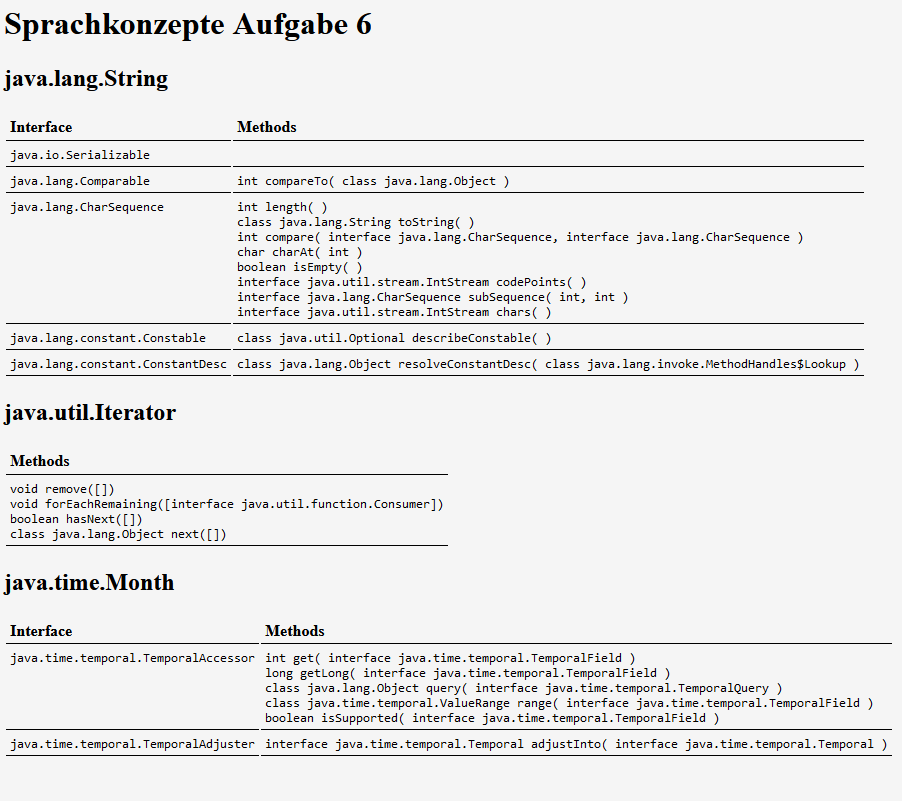
\includegraphics[width=\textwidth]{media/Aufgabe6}
	\caption{Erzeugte HTML-Seite}
	\label{img:Aufgabe6}
\end{figure}
\newline